\section{Projection mapping}

\begin{itemize}
	\item Improvement of gazebo simulator camera implementation to allow modeling of the projection matrix in Ogre3D for accurate projection mapping (sub-millimeter)
	\item Addition of dynamic text, image and video to gazebo simulator for allowing to change the content of the instructions for each assembly step
\end{itemize}


\subsection{Projector modeling}

Over the years, several projection technologies were developed according to the requirements of color fidelity / saturation, image sharpness, brightness, contrast, refresh rate and price. Currently, the video projection market is split between reflective \gls{dlp} and transmissive \gls{lcd} projection technology, with a small percentage of projectors consisting of a hybrid between the two technologies (\gls{lcos}).

For video projection mapping purposes \cite{Raskar1998,Bimber2005,Tan2013,Fujimoto2014}, reflective projectors are better suited than the remaining technologies given their ability to create images with smaller gaps between the projected pixels (smoother images) and they also have higher contrast, better color accuracy / uniformity, much fewer dead pixels and the image quality does not degrade over time. The main stages of the image creation in a \gls{dlp} projector are show in \cref{fig:dlp-projector-diagram-dmd}. The first phase is the generation of light from either a lamp or a \gls{led} / laser array, which is later on condensed on a lens in order to pass through a moving color wheel to become one of the 3 primary additive colors (red, green, blue). The colored light then passes through a shaping lens and hits a \gls{dmd} which has an electronic controllable mirror for each projection pixel that either reflects the light into the projection lens or into a heat sink. Color shading is achieved by controlling how long and how often the micro mirrors in the \gls{dmd} are reflecting each light color into the lens (or into the heat sink).


\begin{figure}[H]
	\begin{floatrow}[2]
		\ffigbox[\FBwidth]
		{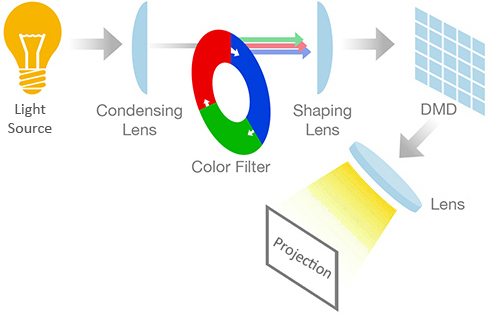
\includegraphics[height=.19\textheight]{dlp-projector-diagram-dmd}}
		{\caption[Single chip \glsentrytext{dlp} diagram]{Single chip \glsentrytext{dlp} diagram\protect\footnotemark}\label{fig:dlp-projector-diagram-dmd}}
		\ffigbox[\FBwidth]
		{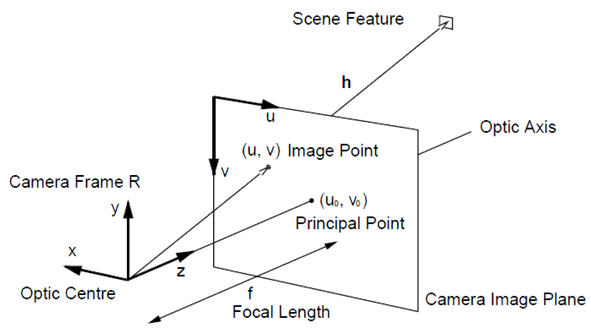
\includegraphics[height=.19\textheight]{camera-intrinsics}}
		{\caption[Pinhole camera model]{Pinhole camera model\protect\footnotemark}\label{fig:camera-intrinsics}}
	\end{floatrow}
\end{figure}
\footnotetext[\the\numexpr\value{footnote}-1\relax]{\url{https://vimeo.com/blog/post/display-tech-home-projectors}}
\footnotetext[\value{footnote}]{\url{http://perso.ensta-paristech.fr/~filliat/Courses/2011_projets_C10-2/BRUNEAU_DUBRAY_MURGUET/monoSLAM_bruneau_dubray_murguet_en.html}}


The mathematical modeling of a \gls{dlp} projector can be seen as an inverse camera, given the grid disposition of the mirrors in the \gls{dmd} and the usage of a lens to focus the light into the projection surface. The galvanometer scanners model is slightly different since there is no lens and no focal point, but it can be approximated by a pinhole camera for efficient scene rendering using \gls{opengl} / Direct3D, with later distortion correction using the mathematical models proposed in \cite{Manakov2011}.

Both projection mapping prototypes modeled the projector with a pinhole camera \cite{Hartley2003} (shown in \cref{fig:camera-intrinsics}) using the \gls{opengl} / Direct3D projection matrix. The matrix formulation for computing the projection matrix is shown in \cref{eq:projection-matrix,eq:ndc-matrix,eq:perspective-matrix}, and it includes the focal lengths (Fx, Fy), principal point (Cx, Cy) and axis skew (S) intrinsic parameters (in pixel units). The correction of lens distortion for \gls{dlp} projectors used 3 coefficients for removing radial distortions and 2 coefficients for accounting for the tangential distortions. The correction of the galvanometer scanners distortion (seen in \cref{fig:laser-projector-diagram-1-colors}) is performed by warping the projection points using the MediaLas LaserCAM application in order to remove the distortion that occurs mainly in the horizontal axis.

{
	\small
	\begin{equation}\label{eq:projection-matrix}
	ProjectionMatrix = \glsentrytext{ndc}Matrix \times PerspectiveMatrix
	\end{equation}
	
	\begin{equation}\label{eq:ndc-matrix}
	NDCMatrix = 
	\begin{bmatrix}
	\frac{2}{ImageWidth} & 0 & 0 & -1 \\
	0 & \frac{2}{ImageHeight} & 0 & -1 \\
	0 & 0 & \frac{-2}{ClipFar - ClipNear} & \frac{-(ClipFar + ClipNear)}{ClipFar - ClipNear} \\
	0 & 0 & 0 & 1
	\end{bmatrix}
	\end{equation}
	
	
	\begin{equation}\label{eq:perspective-matrix}
	PerspectiveMatrix = 
	\begin{bmatrix}
	Fx & S & -Cx & 0 \\
	0 & Fy & -Cy & 0 \\
	0 & 0 & ClipNear + ClipFar & ClipNear \times ClipFar \\
	0 & 0 & -1 & 0
	\end{bmatrix}
	\end{equation}
}


\subsection{Projector calibration}

The intrinsic parameters of a \gls{dlp} projector can be computed using image analysis of complementary gray code patterns (seen in \cref{fig:dlp-calibration-pattern-wall}) projected into a chessboard. The calibration system proposed in \cite{Moreno2012} was used to retrieve the 5 intrinsic parameters (Fx, Fy, Cx, Cy, S) of the projector along with the 3D position and rotation of the projector in relation to the camera. It was used 5 sets of 42 gray code image patterns captured with the chessboard in different positions and orientations in relation to the projector, that was at a distance of 2.2 meters from the table workspace. After calibration it was projected a validation pattern to evaluate the accuracy of the projection, and it can be seen in \cref{fig:dlp-projected-chessboard} that the white squares were projected into the chessboard with sub-millimeter accuracy.

\begin{figure}[H]
	\begin{floatrow}[2]
		\ffigbox[\FBwidth]
		{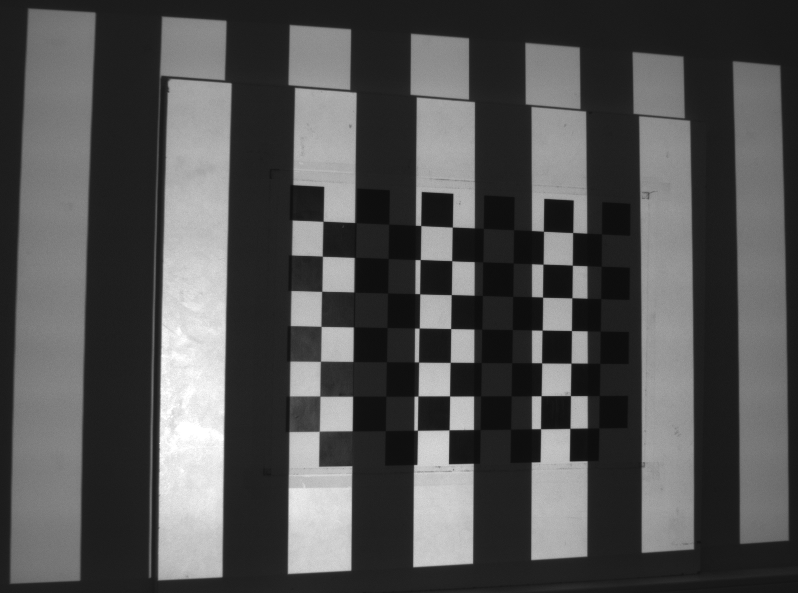
\includegraphics[height=.205\textheight]{dlp-calibration-pattern-wall}}
		{\caption{One of the \glsentrytext{dlp} projector calibration patterns}\label{fig:dlp-calibration-pattern-wall}}
		\ffigbox[\FBwidth]
		{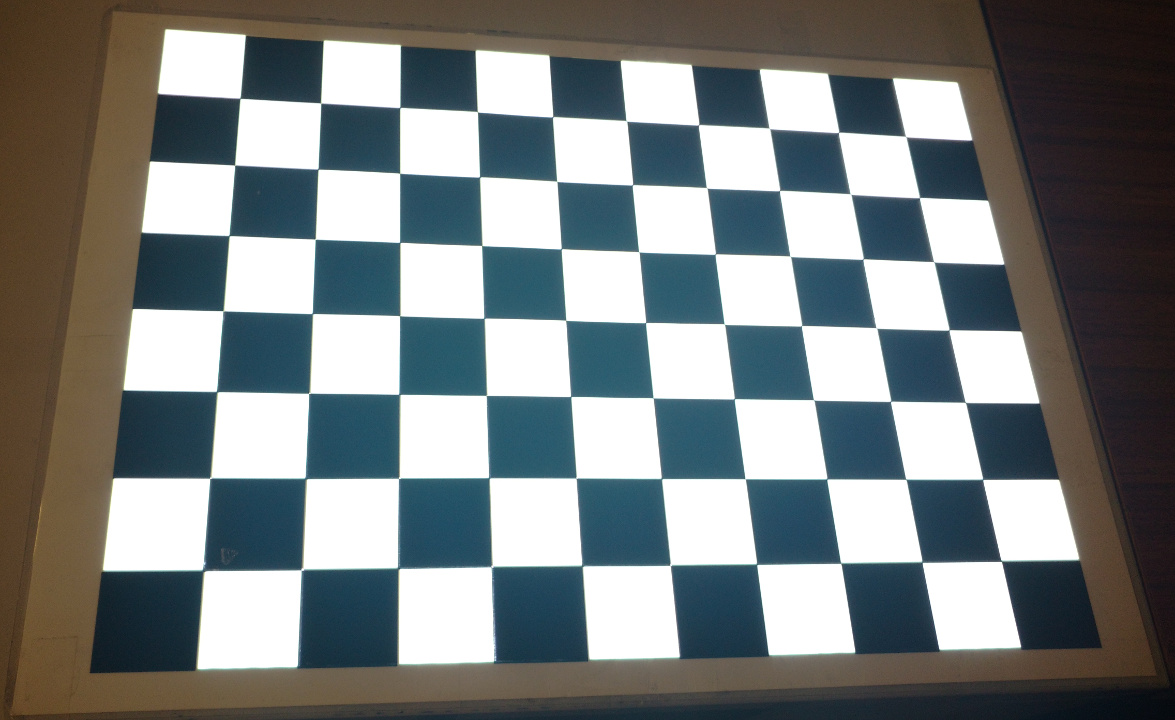
\includegraphics[height=.205\textheight]{chessboard}}
		{\caption{\glsentrytext{dlp} projector validation pattern}\label{fig:dlp-projected-chessboard}}
	\end{floatrow}
\end{figure}


\subsection{Camera extrinsics calibration}

For fast recalibration of the projector 3D position and orientation in the global coordinate system of the workspace, both the \gls{dlp} projector and galvanometer scanner had a 5 \gls{mp} Mako G-503B\footnote{\url{https://www.alliedvision.com/en/products/cameras/detail/Mako\%20G/G-503.html}} camera firmly attached to the projectors support. As such, the global position of the projector is given by multiplying the $4 \times 4$ homogeneous matrix that gives the transformation from the chessboard corner (shown in \cref{fig:chess-board-detection}) to the camera, with the $4 \times 4$ homogeneous matrix that gives the transformation from the camera to the projector.

For the \gls{dlp} projector the camera-to-projector matrix was computed using the software described in \cite{Moreno2012}. For the galvanometer scanner this matrix was calculated by placing the projector at 2 meters from a wall, properly leveled in order to ensure that the laser beam was hitting the wall perpendicularly, and then placing a chessboard in the wall in such a way that the center of projection was hitting one of the chessboard corners. By knowing the projector and camera position / orientation in relation to a known coordinate system (the chessboard origin), the transformation from the camera to the galvanometer scanner can be easily computed using \cref{eq:extrinsics-camera-projector}.

\begin{small}
	\begin{equation}\label{eq:extrinsics-camera-projector}
	CameraToProjectorMatrix = ProjectorToChessboardOrigin \times (CameraToChessboardOrigin^{-1})
	\end{equation}
\end{small}

\begin{figure}[H]
	\centering
	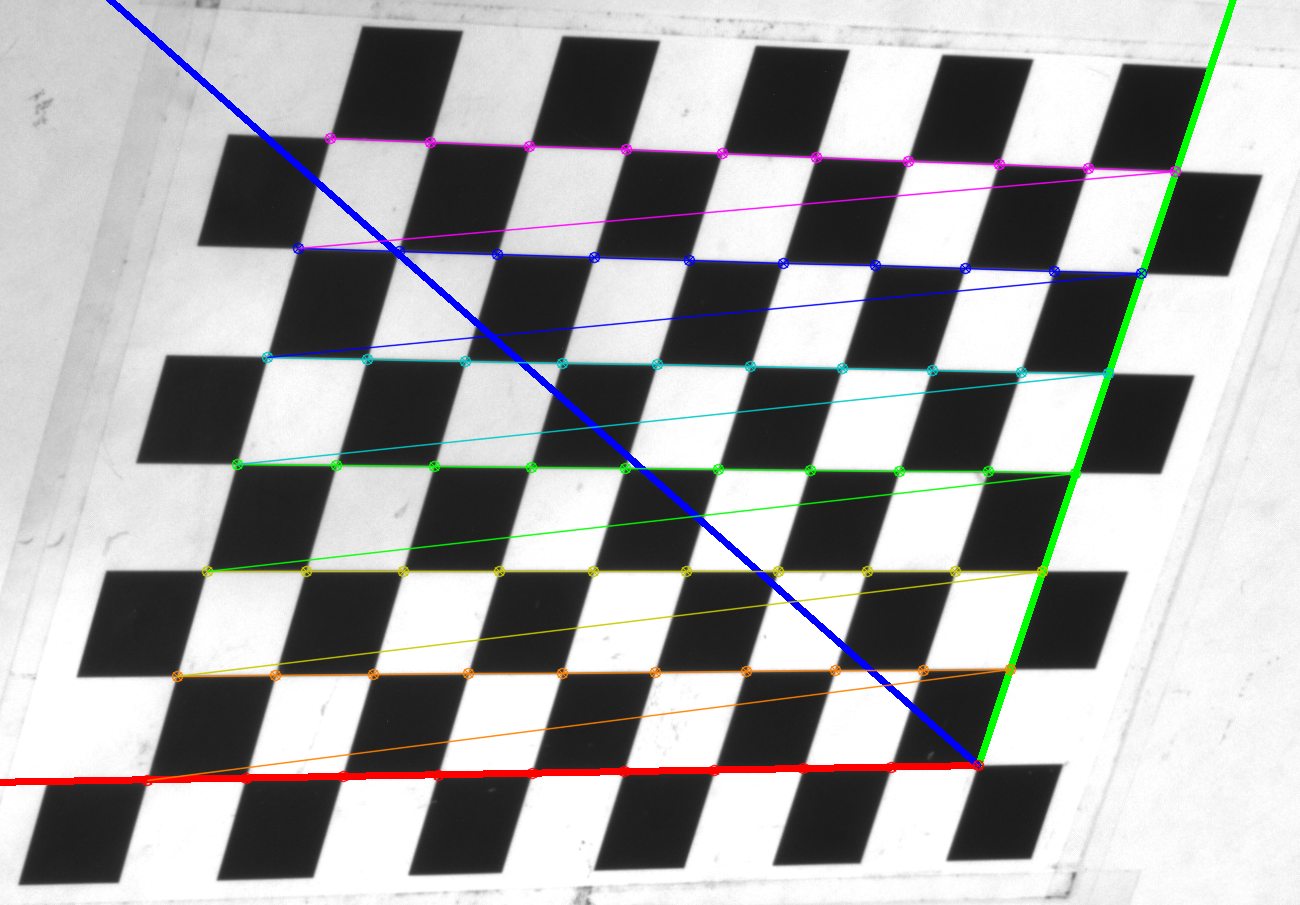
\includegraphics[width=0.47\linewidth]{chess-board-detection}
	\caption{Example of chessboard origin detection}
	\label{fig:chess-board-detection}
\end{figure}


\subsection{Scene rendering}

For efficient scene rendering, both projection mapping prototypes relied on \gls{gpu} \glspl{api} to take advantage of the massively parallel graphics cards currently available. The Gazebo simulator relied on the cross platform open source Ogre3D graphics engine\footnote{\url{http://www.ogre3d.org}} to generate raster images for the \gls{dlp} projectors (example in \cref{fig:dlp-projection-image}), while Eyeshot used the Microsoft proprietary Direct3D rendering engine, which supports native rendering of vector graphics scenes (useful for generating vector images from \gls{cad} models and vector drawings which are required when using galvanometer scanners).

For user interface, the Gazebo simulator allows visual inspection of the scene (shown in \cref{fig:gazebo-user-interface}) while also giving the option to add new objects or move and rotate existing models. The Eyeshot prototype also allows to inspect the scene and has a dedicated interface for validating and adjusting the projector intrinsic and extrinsic parameters (seen in \cref{fig:eyeshot-user-interface-vector-lines}).


\subsubsection{Human machine interaction}

\begin{itemize}
	\item Modeling of the user interaction with the projected interface by defining a set of Regions of Interest (ROIs) in which the 3D sensor data falls
	\item When a minimum number of points falls within a given ROI, the points centroid is extracted and:
	\begin{itemize}
		\item If it is a button, the user needs to hold the finger for 0.2 seconds to trigger the action. Moreover, to avoid unintentional triggering , the user needs to remove the finger from the ROI to trigger the action again
		\item If it is the video seek bar, the video position is computed considering the height of the video and the relative position of the finger in relation to the button of the video
	\end{itemize}
\end{itemize}

\textbf{Supported actions}
\begin{itemize}
	\item Go to the first assembly step
	\item Go to the previous assembly step
	\item Go to the next assembly step
	\item Go to the last assembly step
	\item Pause the video
	\item Change the position of the video (seek)
\end{itemize}

\begin{figure}
	\centering
	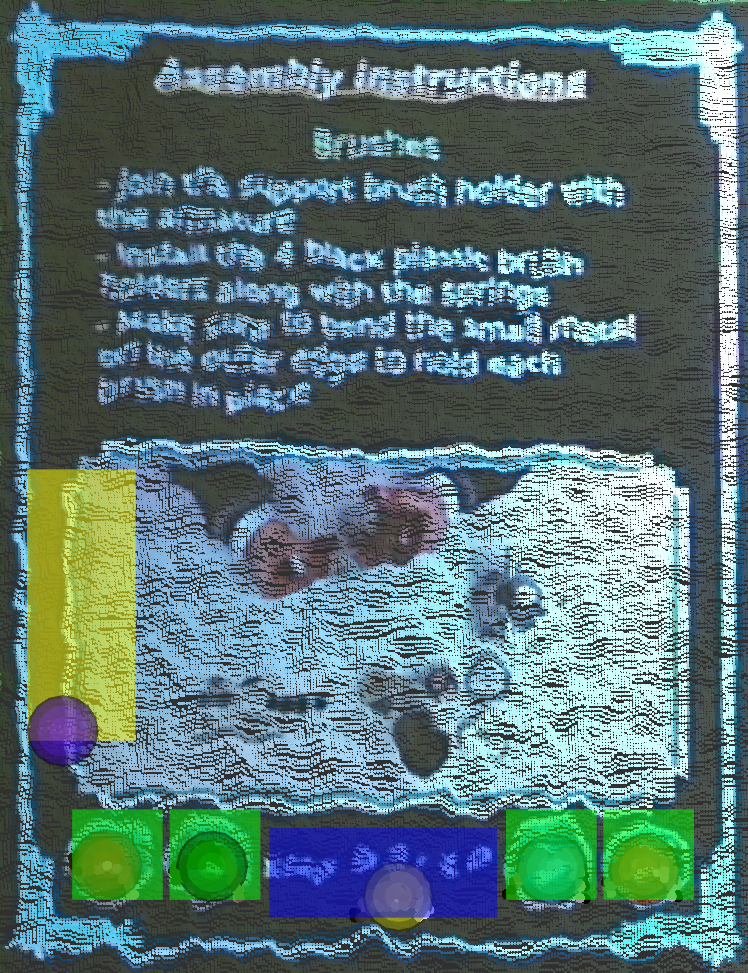
\includegraphics[width=0.4\linewidth]{interaction-rois}
	\caption{Regions of interest for the human machine interaction interface}
	\label{fig:interaction-rois}
\end{figure}



\subsubsection{Object 3D reconstruction}

\begin{itemize}
	\item Usage of the David Laser structured light system to obtain the 3d mesh model of the assembled object (no CAD was available)
\end{itemize}

\begin{figure}[ht]
	\centering
	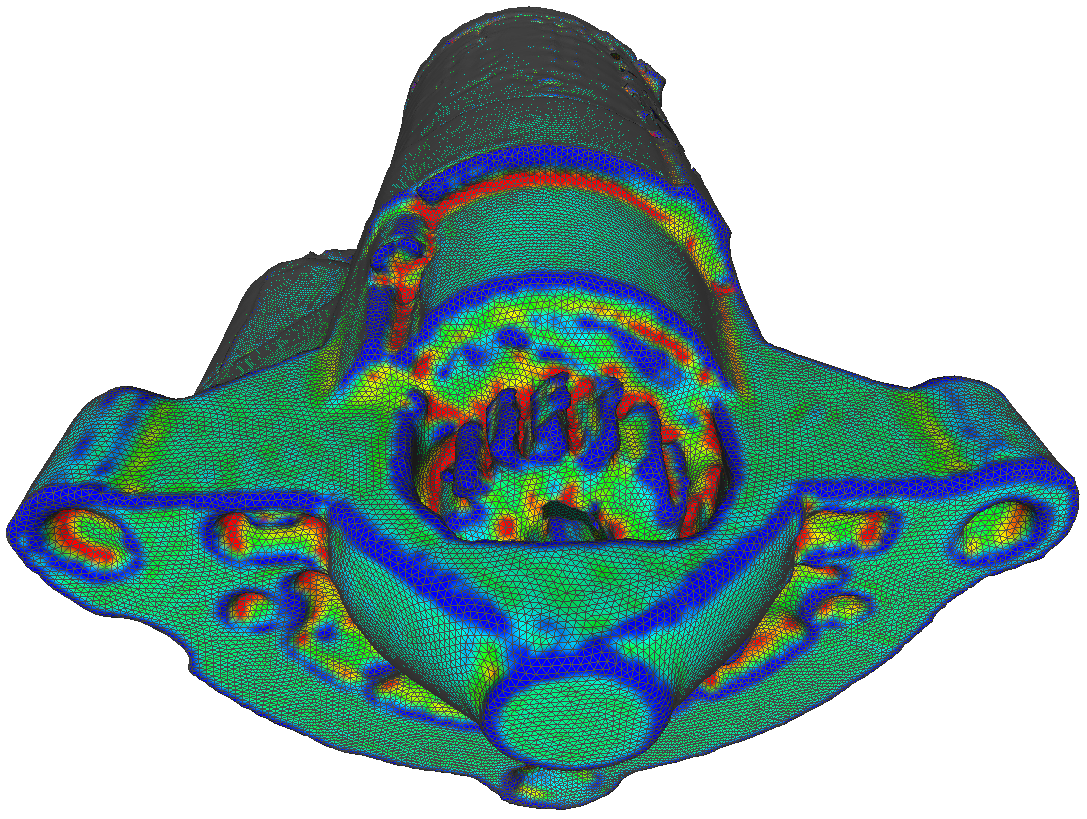
\includegraphics[height=.25\textheight]{object-reconstruction-back}
	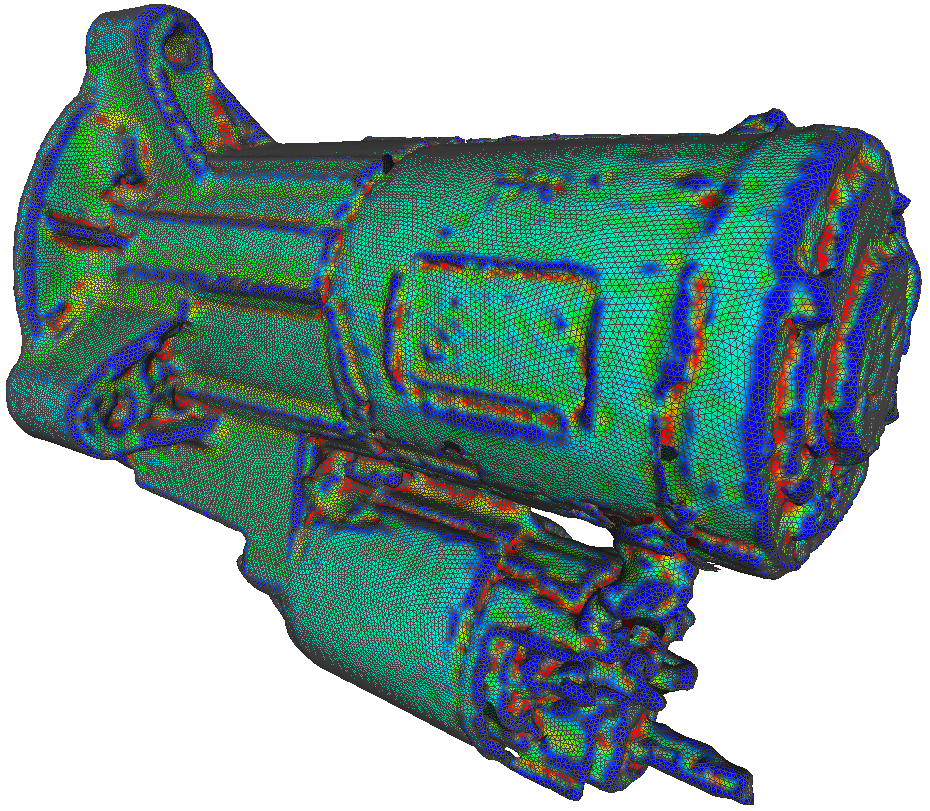
\includegraphics[height=.25\textheight]{object-reconstruction-front}
	\caption{3D model of the starter motor reconstructed using structured light}
\end{figure}


\subsubsection{Object recognition}

\begin{itemize}
	\item 6 DoF initial pose estimation using:
	\begin{itemize}
		\item 3D SIFT keypoint detector
		\item Fast Point Feature Histogram (FPFH) descriptor
		\item Estimation of the best point cloud initial registration using a Random Sample Consensus (RANSAC) approach
		\item Refinement of the initial pose estimation using Iterative Closest Point (ICP)
	\end{itemize}
	\item After the initial pose estimation, the object pose is tracked using only ICP (no need for feature detection and estimation)
\end{itemize}

\begin{figure}[!ht]
	\centering
	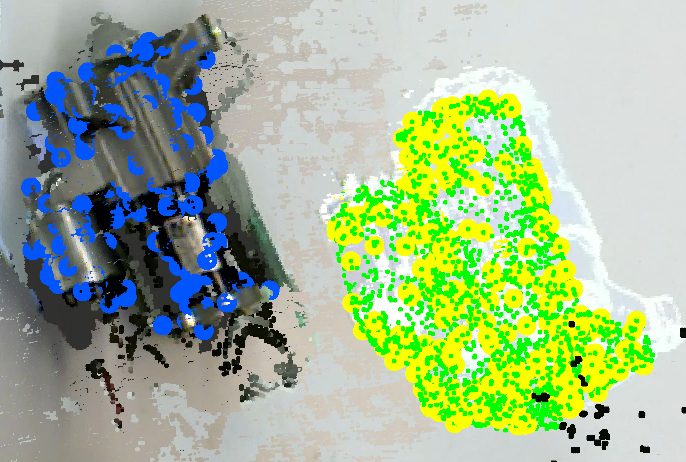
\includegraphics[height=.27\textheight]{initial-pose-estimation-1-before}
	\hspace{0.5em}
	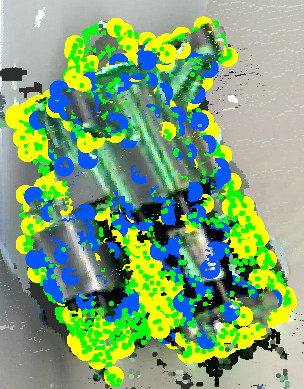
\includegraphics[height=.27\textheight]{initial-pose-estimation-1-after}
	\caption{Initial pose estimation of assembled object}
\end{figure}

\begin{figure}[!ht]
	\centering
	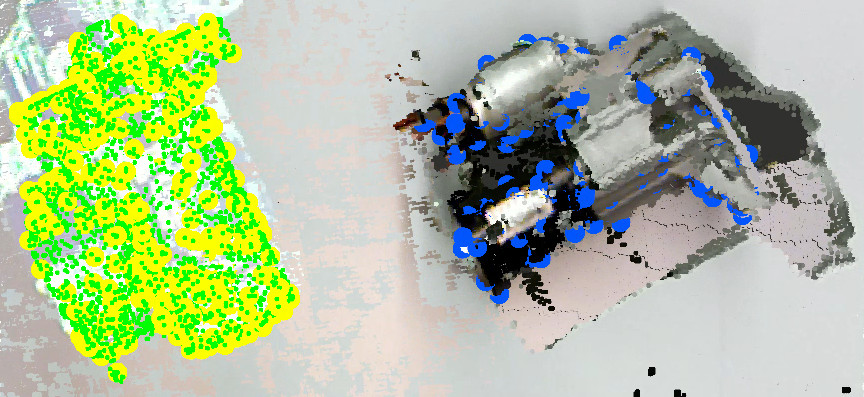
\includegraphics[height=.182\textheight]{initial-pose-estimation-2-before}
	\hspace{0.5em}
	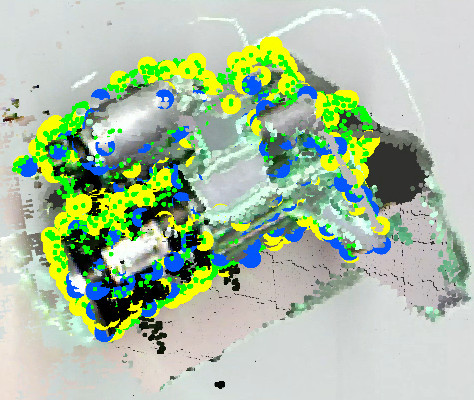
\includegraphics[height=.182\textheight]{initial-pose-estimation-2-after}
	\caption{Initial pose estimation of assembled object}
\end{figure}
